\section{Iteration 4: Decomposition of the Storage Unit}
\label{add:it4}

\subsection{Step 1: Identify candidate drivers}
\label{add:it4/drivers}

\npar This iteration is driven by

\begin{itemize}
	\item Av1: Measurement database failure. The measurements database should be up
	and running 99.9\% of all time. 
  	\item P3': Requests to the measurement database. The requests should be
  	handled within a bounded time. 
\end{itemize}

\npar There are two delegated (and split) use cases:

\begin{itemize}
  	\item UC8' : Send measurement. measurements need to be stored.
  	\item UC17' : Perform research. researchers should be able to query the
  	database.
\end{itemize}

\subsection{Step 2: Choose design concepts}
\label{add:it4/concepts}

\subsubsection{Tactics}
\label{add:it4/tactics}

\paragraph{Availability} 

\npar Av1 states that a 99.9\% uptime must be realized. In order to guarantee
this, three things must be taken into consideration. It should be able to detect
the problem, there should be a way to fix the problem and last but certainly not
least, there should be preventive measures.

\npar There are many alternatives to address availability. The most frequently
used ones are active redundancy, passive redundancy and the use of spares (hot
or cold). The main criterion to select one of these is the time it takes to
recover. This time is respectively in the order of milliseconds, seconds and
minutes. An uptime of 99.9\% corresponds to 0.72 hours (or 43.2 minutes) of
permitted downtime on a monthly basis. 

\npar The use of spares is probably not the best option. Even though the
effective time of replacement is unknown, one can assume it will take quite some
time to replace an important element such as the measurements database. Based on
that time, the number of crashes will be low or even zero. For this reason, use
of spares is eliminated.

\npar The difference between active and passive replication is rather subtle.
In an active replication scheme, the system will recover faster then in a
passive replication scheme but all replicas should be in a consistent
state. This, however, increases synchronization overhead in comparison with
the passive replication scheme.

\npar On the other hand, the active replication scheme can also provide load
balancing for read-only queries. If one replica has a lower load than any other,
that replica can be used to process the query. Because of this advantage, the
active replication scheme is selected.

\subsubsection{Design Patterns}
\label{add:it4/patterns}

\paragraph{Replicated Component Group} 

\npar To make the data highly available, the database will be replicated. This
can be achieved by using the \emph{Replicated Component Group} design pattern
\citep[see][p.~326]{Buschmann:07}. A single instance is replaced by the
component interface and the implementation is replicated among a number of
nodes. Because of the increased fault-tolerance, it will also increase availability.

\paragraph{Business Delegate}

\npar The \emph{Business Delegate} design pattern
\citep[see][p.~292]{Buschmann:07} can be used to make communication with
replicas transparent. The delegate can implement the component interface of the
replicated component group and serve as a front end for all actions on the
replicated instances.

\subsection{Step 3: Instantiate architectural elements and allocate responsibilities}
\label{add:it4/elements}

\npar A business delegate, called MeasurementStorageFrontEnd, will provide an
interface to execute queries on the measurements database. This database will be
replicated among different nodes, called MeasurementStorageInstances. The
FrontEnd will coordinate interaction between all storage instances and will also
manage references to a buffer, called TemporaryBuffer, for temporary storage of
measurement trames in case the database becomes unavailable and a cache, called
MeasurementStorageCache, to speed up requests to the measurements database in
case to load is high.

\npar An overview of the child components is shown in figure
\ref{fig:it4/elements}.

\begin{figure}[H]
	\begin{centering}
		% TODO Figure
		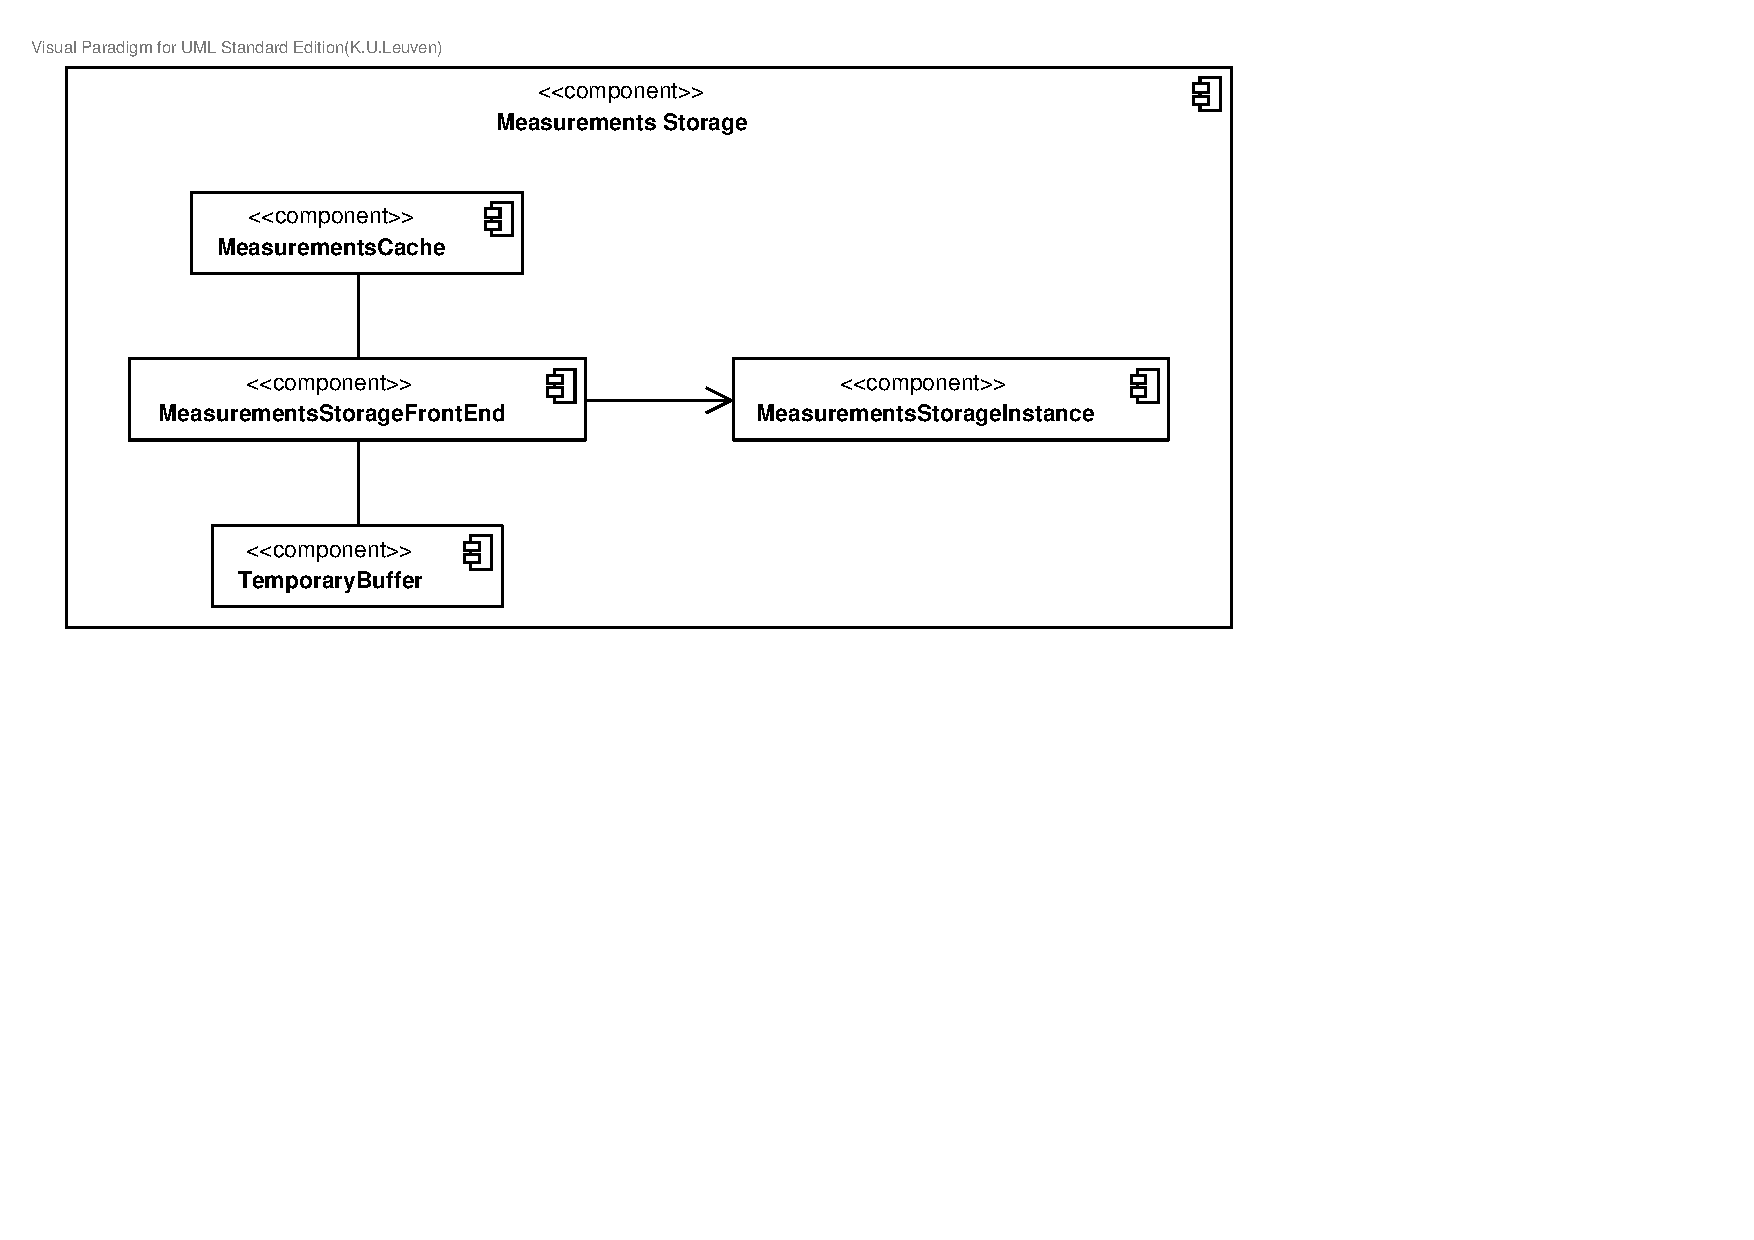
\includegraphics[width=\textwidth]{figs/add-it4-elements.pdf}
		\caption{Overview of all instantiated child elements in the Measurement
		Storage}
		\label{fig:it4/elements}
	\end{centering}
\end{figure}

\subsection{Step 4: Define interfaces for instantiated elements}
\label{add:it4/interfaces}

\subsubsection{MeasurementStorageFrontEnd}

\npar The MeasurementStorageFrontEnd component provides an interface
\interface{MeasurementStorageAPI} to the Measurements Scheduler. This interface
contains one method \method{execute(QueryCommand)} that offers a way
to execute a query on the measurements database. The Query is encapsulated as an
object. A Callback is provided within that object in order to present the
results of the query to the issuer when the query is executed.

\subsubsection{MeasurementStorageInstance}

\npar The MeasurementStorageFrontEnd does not contain the data. It delegates
the queries to one or more MeasurementStorageInstances through the
\interface{MeasurementStorageInstanceAPI} interface. This interface contains a
a synchronous method \method{execute(Query)}. Both the query and the
result are encapsulated in objects.

\npar Apart from the \method{execute()} method, additional methods are provided
for monitoring the load on all instances.

\subsubsection{MeasurementStorageCache}

\npar The MeasurementStorageCache provides an interface
\interface{MeasurementStorageCacheAPI}, similar to the
\interface{MeasurementStorageInstanceAPI}. It has the same method definition for
executing queries. 

\subsubsection{TemporaryBuffer}

\npar The TemporaryBuffer offers an \interface{TemporaryBufferAPI} interface
which contains methods for adding and removing QueryCommands. 

\npar The method \method{add(QueryCommand)} add a QueryCommand to the end
of the buffer and the method \method{remove()} removes the first
QueryCommand from the buffer.

\npar An overview of all child components and their interfaces is shown in
\ref{fig:it4/interfaces}.

\begin{figure}[H]
	\begin{centering}
		% TODO Figure
		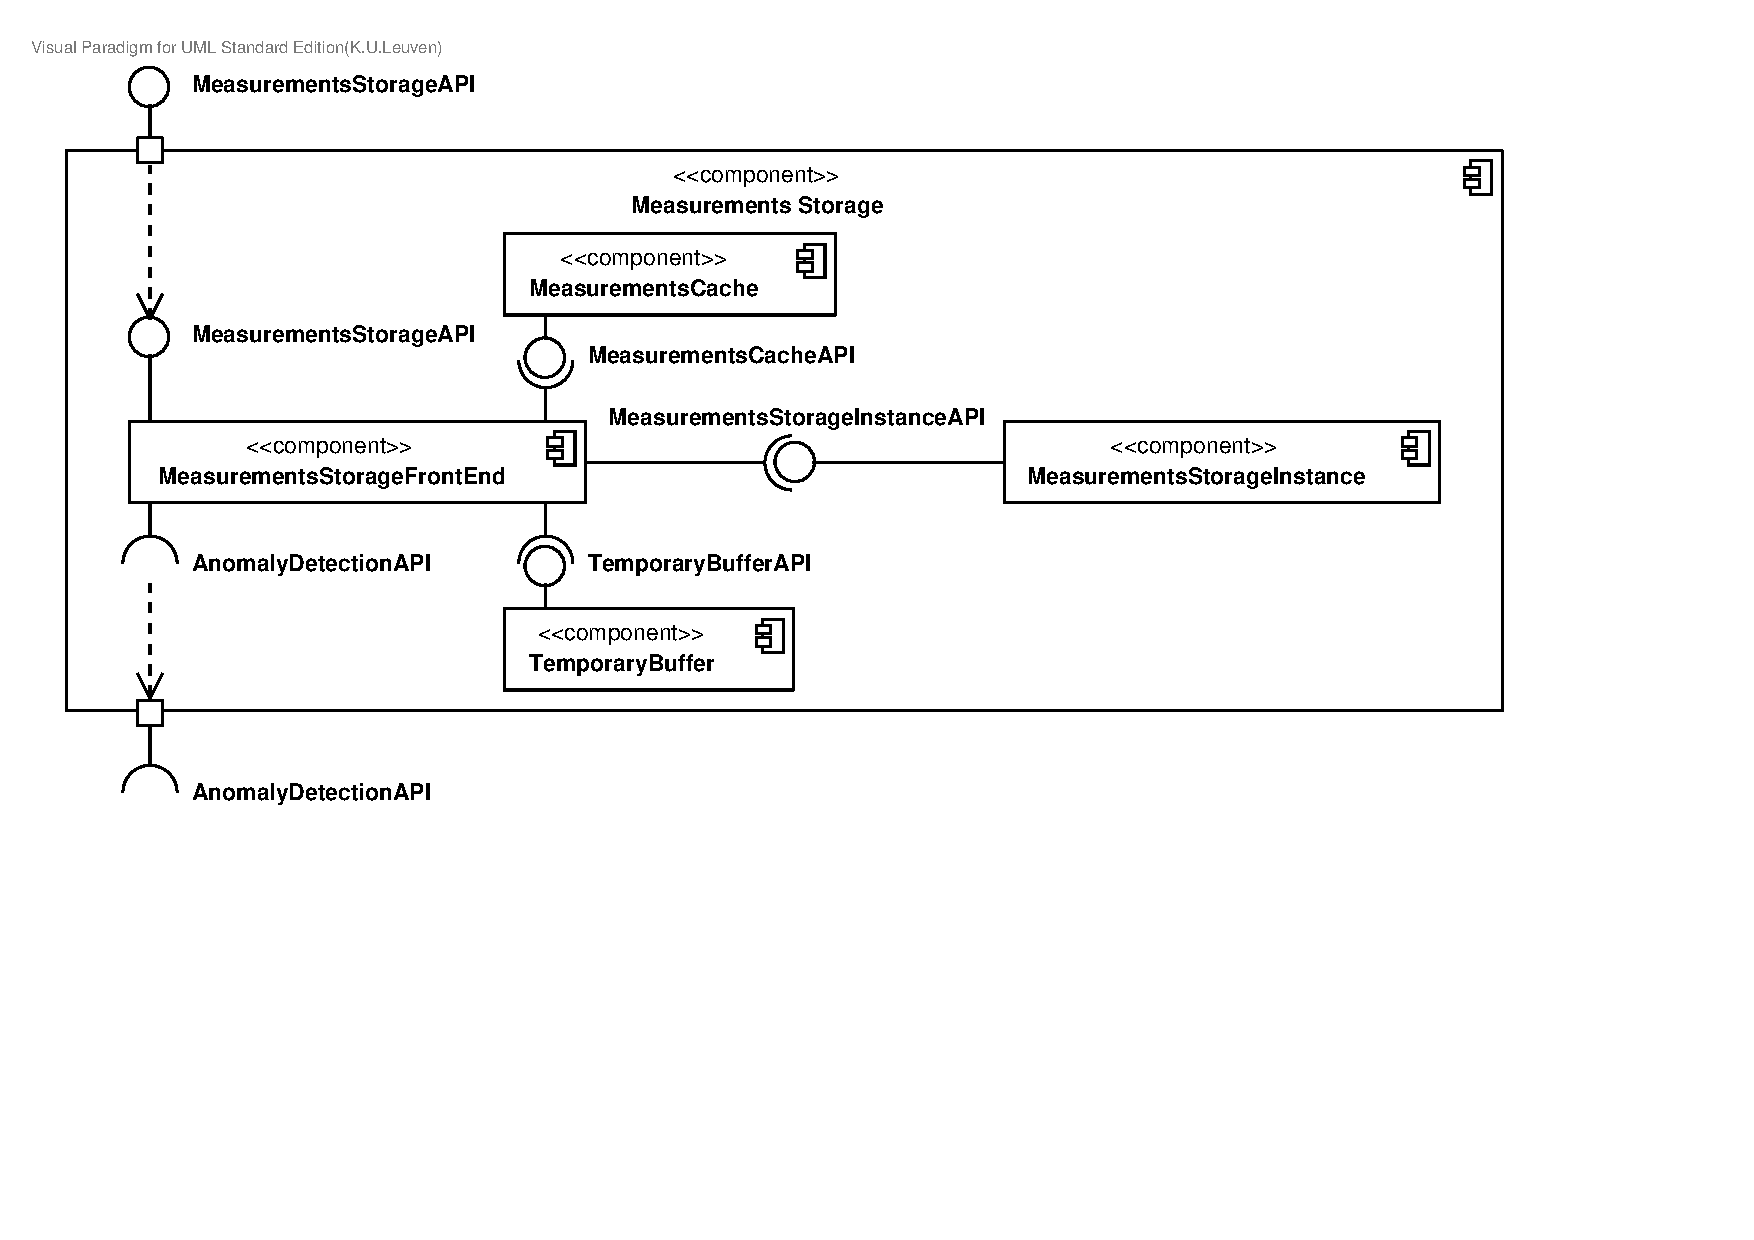
\includegraphics[width=\textwidth]{figs/add-it4-interfaces.pdf}
		\caption{Overview of the interfaces and components in the Measurement Storage}
		\label{fig:it4/interfaces}
	\end{centering}
\end{figure}

\subsection{Step 5: Verify and refine}
\label{add:it4/verification}

\npar All quality requirements are met in this iteration. The database is
replicated for availabililty and this replication potentially also yields a
speed improvement for read queries by using load balancing across database
instances.
